\documentclass[11pt, a4j]{jreport}

\usepackage{comment}
\usepackage{float}
\usepackage{color}
\usepackage{multicol}
\usepackage[dvipdfmx]{pict2e}
\usepackage{wrapfig}
\usepackage{graphicx}
\usepackage{bm}
\usepackage{url}
\usepackage{underscore}
\usepackage{colortbl}
\usepackage{tabularx}
\usepackage{fancyhdr}
\usepackage{ulem}
\usepackage{cite}
\usepackage{amsmath, amssymb, amsfonts}
\usepackage{algorithmic}
\usepackage{textcomp}
\usepackage{xcolor}
\usepackage[ipaex]{pxchfon}

\usepackage[top=30truemm, bottom=30truemm, left=25truemm, right=25truemm]{
    geometry
}

\begin{document}
    \thispagestyle{empty}
    \begin{center}
        \vspace{20mm}
        {\Large\noindent 2024年度 卒業(学士)論文}\\
        \vspace{40mm}
        {\huge\noindent\textbf{SNSにおける世論形成と紛争に関するReddit投稿分析}}\\
        \medskip
        {\huge\noindent\textbf{ーイスラエルによるレバノン侵攻を例にー}}\\
        \vspace{\baselineskip}
        \vspace{40mm}

        {\Large\noindent 2025年1月31日\\ \vspace{\baselineskip} 指導教員 崎田智子 \\ \vspace{\baselineskip} 同志社大学\\ グローバル地域文化学部グローバル地域文化学科アジア・太平洋コース \\ \vspace{\baselineskip} 1122192047 種村尚大\\ }
        \vspace{40mm}
    \end{center}

    \thispagestyle{empty}
    \clearpage

    %=====================================================================================
    \renewcommand{\abstractname}{要旨}

    \begin{abstract}
        研究の要旨。なんやかんやなんやかんやなんやかんやなんやかんやなんやかんやなんやかんやなんやかんやなんやかんやなんやかんやなんやかんやなんやかんやなんやかんやなんやかんやなんやかんやなんやかんやなんやかんやなんやかんやなんやかんやなんやかんやなんやかんや
    \end{abstract}

    %=====================================================================================

    % 目次の表示
    \tableofcontents

    %=====================================================================================
    \pagestyle{fancy}
    \lhead{\rightmark}
    \renewcommand{\chaptermark}[1]{\markboth{第\ \normalfont\thechapter\ 章~~#1}{}}
    %=====================================================================================

    \chapter{はじめに} %章

    \section{研究背景} %1.1
    21世紀における紛争の展開は、これまでの軍事的な衝突だけでなく、情報空間における戦いも大きな意味を持つようになっている。中でも、ソーシャルネットワーキングサービス(SNS)は紛争のリアルタイムでの情報発信や世論形成において強い影響力を持っている。特にRedditのような匿名性と多様な意見交換が可能なプラットフォームは、国際的な出来事に対する個人の反応を即座に可視化する場として機能している。

    近年、再び激化したイスラエルとハマス間の戦闘は、デジタル空間における議論にも大きな影響を及ぼしている。1948年のイスラエル建国以来、パレスチナ人の土地権利や自治権、イスラエルの安全保障、エルサレムの帰属問題など、複雑な歴史的背景が絡むこの対立は、度重なる衝突と共に深刻さを増している。特に2023年10月7日のハマスによる襲撃とその後の戦闘激化は、国際メディアだけでなくSNSでも大きな反響を呼び、一般市民やアクティビストが活発に意見や情報を発信するようになった。この対立は2024年10月1日、イスラエルのレバノン侵攻という形で地域的な拡大を見せ、人道危機への懸念と共にSNS上での議論も一層活発化した。Redditはこの一連の動きを捉える重要な場として機能し、紛争の展開や人道状況に対する人々の反応を観察できる貴重な分析対象となっている。Reddit上の投稿数や内容の変化を観察することで、現代の紛争がどのようにデジタル空間で議論され、どのようなトピックが注目されるのかを理解するための重要な手がかりが得られる。

    \section{研究目的}
    本研究の目的は、2024年10月1日のイスラエルによるレバノン侵攻がReddit上でどのように反映されたかを分析することにある。特に、侵攻発生直後の投稿数の変動、および特定のテーマ(例:戦争犯罪、人道的危機、政治的意見)の頻出度の変化に焦点を当てる。本研究は、現代の紛争に対するオンラインコミュニティの反応を解析し、SNSが世論や情報戦に与える影響について新たな知見を提供することを目指している。

    この研究の独自性は以下の点にある:

    \begin{enumerate}
        \item Redditという特定のプラットフォームに焦点を当て、その特異性(匿名性、サブレディット構造)が国際紛争に関する議論にどのような影響を与えるかを明らかにする。

        \item 大規模なデータ分析と質的分析を組み合わせることで、単なる投稿数の変化だけでなく、議論の質的変化も捉える。

        \item 紛争勃発直後の短期的な反応から、長期的な議論の推移まで、時系列での変化を詳細に分析する。
    \end{enumerate}

    本研究で取り上げる仮説は以下の通りである:

    \begin{enumerate}
        \item レバノン侵攻が発生すると、Reddit上の投稿数は急増し、議論は一時的に過激化する傾向がある。

        \item Redditの各サブフォーラムでは異なる視点や意見が展開され、一部では紛争の当事者に対する支持や批判が顕著に表れる。

        \item 戦闘の継続期間に伴い、投稿の焦点は戦闘に関する最新情報から、被害者支援や国際的な対応策にシフトしていく。
    \end{enumerate}

    \section{本論文の構成}
    本論文は、以下の構成で進める。第2章では、SNSにおける世論形成と国際紛争に関する先行研究をレビューし、Redditが持つ特異な役割について検討する。第3章では、Reddit上での投稿データを収集し、投稿数や内容の変化を定量的に分析するための方法論を説明する。第4章では、データ分析の結果を提示し、第5章でその結果を考察することで、SNSにおける紛争に対する反応のメカニズムについて洞察を得る。最後に、第6章では本研究のまとめと今後の課題を述べる。

    本研究は、現代の紛争に対するオンラインコミュニティの反応を解析することで、SNSが世論や情報戦に与える影響について新たな知見を提供することを目指している。これにより、デジタル時代における国際紛争の理解と対応に貢献することが期待される。

    \chapter{SNSにおける世論形成と国際紛争に関する先行研究}

    \section{SNSと世論形成}
    ソーシャルネットワーキングサービス(SNS)は、21世紀において世論形成における重要なツールとなり、従来のマスメディアと比較して情報が広範に、瞬時に拡散されるという特性を持つ。Shirky(2011)は、SNSを「集団行動を促進するツール」として位置づけ、情報の共有と協働に着目している。この見解は、2010年代の「アラブの春」などの社会運動におけるSNSの役割を説明する上で重要な視点を提供している。

    特に、SNSは政治的・社会的な問題に対する迅速な反応を引き出す手段として機能しており、従来のメディアでは捉えられなかった多様な声を可視化している。例えば、TwitterやFacebookなどのSNSプラットフォームでは、短期間で広範に拡散された情報が瞬時に世論形成に影響を与える。このようなプラットフォームの役割は、選挙、社会運動、または緊急時における意思決定に大きな影響を与えている。

    一方で、SNSにおける情報の流通には批判的な見方も存在する。Sunstein(2001)とPariser(2011)は、SNSにおける同調バイアスやエコーチェンバー現象の危険性を指摘している。これらの現象により、ユーザーは自身の既存の見解を強化する情報のみに接触し、多様な意見に触れる機会が減少する可能性がある。この批判は、SNSが真の意味での対話や意見の多様性を促進しているかという疑問を投げかけている。

    \section{国際紛争におけるSNSの役割}
    国際紛争において、SNSは「デジタル戦場」として利用されることが増加している。HowardとHussain(2013)は、アラブの春やシリア内戦におけるSNSの役割について、プロテスタントが情報を共有し、活動を組織化する手段として重要な機能を果たしたと指摘している。これにより、紛争に関する情報操作やプロパガンダがSNSを通じて行われ、情報がリアルタイムで拡散される現象が確認されている。この研究は、SNSが単なる情報共有の場を超えて、実際の社会変革や紛争の展開に直接的な影響を与え得ることを示している。

    加えて、SNSは国際機関やニュースメディアの報道を補完し、個人レベルでの意見発信や反応を可視化する重要なプラットフォームとなっている。特に、イスラエルとパレスチナの紛争では、世界中のユーザーがSNSを通じて意見を表明し、国際的な議論が加速している。このようなSNS上の情報流通は、紛争の当事者に対するプレッシャーや外交的アプローチに影響を与えることがある。

    Zeitzoff(2017)は、イスラエル・ハマス紛争におけるTwitterの役割を分析し、SNSが紛争当事者の戦略的コミュニケーションと世界的な支持獲得の場として機能していることを明らかにした。この研究は、SNSが紛争の「ソフトパワー」的側面において重要な役割を果たしていることを示唆している。

    また、BennettとSegerberg(2012)によれば、SNSは「ネットワーク化された個人的行動」を促進し、従来の組織化されたプロテスト運動とは異なり、より分散的かつ迅速に多くの個人を結びつける力を持つ。この視点は、国際紛争におけるSNSの役割が、単なる情報の伝達を超えて、個人の行動を直接的に動員する可能性を示唆している。

    \section{Redditの特異性}
    Redditは他のSNSと比較して匿名性が高く、ユーザーが個別のトピックに関心を持つコミュニティ(サブレディット)に参加する構造を持っている。Massanari(2015)によれば、Redditの匿名性と分散型構造が、他のSNSとは異なる形で多様な意見交換を可能にしている。また、Redditの「アップボート」および「ダウンボート」の評価システムは、コンテンツの可視性をユーザーによる評価に委ねるものであり、多様な視点や意見が反映されやすいプラットフォームとなっている。

    この評価システムは、多数派の意見が上位に表示される一方で、論争的な意見や少数派の見解も一定の支持を得て拡散される可能性がある。また、Redditには多様なサブレディットが存在し、国際ニュースに対する一般的な議論が展開される「r/worldnews」や「r/politics」のようなサブフォーラムに加え、特定の地域やテーマに特化したサブレディットも存在する。これにより、同じ紛争に対しても異なる視点からの議論が展開されることが多い。

    GaffneyとMatias(2018)の研究では、Redditのコメントシステムが階層的な議論の構造を生み出し、これが複雑な議題設定や意見形成のプロセスを促進することが示されている。この特徴は、国際紛争のような複雑な問題に対して、多層的な議論を可能にする潜在性を持っている。

    また、Mills(2018)は、Redditのサブレディットが「想像の共同体」として機能し、特定のイデオロギーや世界観を共有するユーザー間の結束を強化する傾向があることを指摘している。この知見は、国際紛争に関する議論がReddit上でどのように展開され、特定の見解が強化されていく可能性があるかを理解する上で重要である。

    \section{先行研究との関係}
    これまでの研究では、SNSが世論形成や政治的動員に与える影響について多くの議論がなされてきたが、特定のSNSプラットフォームに焦点を当てた研究は相対的に少ない。特に、Redditのような匿名性の高いプラットフォームにおける世論形成や紛争に対する議論の展開については十分な分析が行われていない。

    本研究は、このギャップを埋め、SNSが国際紛争における意見形成に与える影響を明らかにすることを目的とする。特に、Redditの特異性(匿名性、サブレディット構造、投票システム)が、ハマス・イスラエル紛争のような複雑な国際問題に対する議論にどのような影響を与えるかを詳細に分析する。これにより、SNSにおける世論形成のメカニズムをより深く理解し、デジタル時代における国際紛争の新たな側面を明らかにすることが期待される。

    \chapter{データ収集・分析手法}
    本章では、Redditにおける投稿データを用いたデータ収集および分析手法について詳述する。データ収集手法は、信頼性と精度を確保しつつ、大規模な投稿データを効率的に取得するためのアプローチを採用する。また、収集されたデータに基づく定量的および定性的な分析手法を理論的に説明し、選択した手法が本研究の目的に対してなぜ有効であるのかを論じる。

    \section{データ収集の方法}
    \subsection{PRAWおよびPushshift APIを用いたデータ収集}
    RedditのAPIであるPRAW (Python Reddit API Wrapper) で大規模な投稿データを効率的に収集する。具体的には、イスラエルによるレバノン侵攻(2024年10月1日)前後の動向を探るため、2024年7月23日から2024年10月23日までの3ヶ月間のデータを収集する。この期間設定により、紛争勃発直後の急激な反応から、その後の議論の推移まで包括的に分析することが可能となる。

    収集対象となるサブレディットは、r/Israel、r/Palestine、r/IsraelPalestineの3つとする。これらのサブレディットは、イスラエル・パレスチナに関する議論が活発に行われている場所であり、異なる視点や立場からの意見を収集することができる。

    \section{定量的分析手法}
    投稿数の時間変化を可視化し、紛争の進展に伴う関心の変動を分析する。具体的には、Pythonのmatplotlibやseabornを用いて、1日ごとの投稿数の推移をグラフ化する。また、レバノン侵攻との対応関係を検証するため、このイベントをタイムラインに組み込む。

    さらに、差分の差分分析(DID)を用いて、紛争関連サブレディットと対照群(r/ps4homebrew、r/Exercise、r/voyageons)との間で投稿数の変化を比較する。DIDモデルの式は以下の通りである:

    \begin{equation}
        Y[it] = β_{0}+ β_{1}* Treatment[i] + β_{2}* Post[t] + β_{3}* (Treatme nt[
        i] * Post[t]) + ε[it]
    \end{equation}

    ここで、$Y[it]$は投稿数、$Treatment[i]$は紛争関連サブレディットか否か、$Post[
    t]$は紛争勃発後か否かを示す。$β_{3}$が紛争の影響を示す推定値となる。

    \subsection{テーマごとの投稿割合の変化}
    トピックモデリング手法としてLDA(潜在ディリクレ配分)を用い、投稿内容のテーマ分類を行う。Pythonのgensimライブラリを使用し、以下の手順で分析を進める:

    \begin{enumerate}
        \item テキストデータの前処理(トークン化、ストップワード除去、ステミング)

        \item 文書-単語行列の作成

        \item LDAモデルの構築(トピック数の設定、ハイパーパラメータの調整)

        \item 各投稿のトピック割り当て

        \item 各トピックの投稿割合の時間変化の可視化
    \end{enumerate}

    これにより、紛争に関する議論のテーマがどのように変遷していくかを定量的に把握する。

    \section{定性的分析手法}
    \subsection{テキスト内容の感情分析}
    VADERセンチメント分析ツールを用いて、投稿の感情極性(ポジティブ、ネガティブ、中立)を分類する。さらに、TextBlobを併用することで、感情分析の結果の信頼性を高める。両ツールの結果を比較し、一致度の高い投稿のみを分析対象とすることで、より信頼性の高い感情分析を実現する。

    感情スコアの時系列変化を可視化し、紛争の進展に伴う感情の変化を追跡する。特に、重要なイベント(例:停戦合意、民間人被害の報道)前後での感情の急激な変化に注目し、これらのイベントがReddit上の議論にどのような影響を与えたかを考察する。

    \subsection{キーワードやフレーズの頻出度解析}
    Pythonのnltkライブラリを使用し、N-gram分析($N=1,2,3$)を行う。これにより、単一の単語だけでなく、複数の単語からなるフレーズの頻出度も分析する。特に注目するキーワードやフレーズには以下のようなものが含まれる:

    \begin{itemize}
        \item 「war crime」「human rights」「civilian casualties」

        \item 「two-state solution」「peace process」「international law」

        \item 「media bias」「propaganda」「fake news」
    \end{itemize}

    これらの頻出度の時系列変化を追跡し、議論の焦点がどのように推移していくかを分析する。また、各サブレディット間での使用頻度の差異を比較することで、コミュニティごとの関心の違いを明らかにする。

    \section{分析手法の有効性}
    本研究で採用した定量的および定性的な分析手法は、Redditにおけるユーザーの反応を多角的に捉えることを目的としている。それぞれの分析手法が持つ有効性を以下に論じる。

    \subsection{定量的分析手法の有効性}
    定量的分析手法は、大規模なデータセットに対して統計的な傾向を明確に示すことができる。特に投稿数の時間系列分析やテーマごとの投稿割合の変化は、紛争に関連するユーザーの関心がどのように推移しているかを直感的に示すことができる。

    DID分析を用いることで、因果関係の特定が可能となり、紛争やその他の外部要因がReddit上での議論の変化にどの程度寄与しているかを厳密に評価できる。この手法は、社会科学研究において広く認められており、本研究のような自然実験的状況下での分析に特に適している。

    さらに、LDAを用いたトピックモデリングは、人間の主観に頼らずに大量のテキストデータから潜在的なテーマを抽出できる点で有効である。これにより、研究者の予見にとらわれない、データ駆動型の分析が可能となる。

    \subsection{定性的分析手法の有効性}
    定性的分析は、定量的分析で示された傾向の背景にある具体的な内容を深く掘り下げる手法として有効である。特に感情分析やキーワードの頻出度解析を通じて、ユーザーが投稿の中でどのような感情や意図を持って情報を発信しているかを理解することができる。

    VADERとTextBlobを併用した感情分析アプローチは、単一のツールを使用する場合と比較して、より信頼性の高い結果を得ることができる。これは、特に皮肉や文脈依存の表現が多いSNS上のテキストデータの分析に有効である。

    また、N-gram分析を用いたキーワードやフレーズの頻出度解析は、単に単語の出現頻度を数えるだけでなく、より複雑な概念や表現の使用傾向を把握することができる。これにより、ユーザーの思考や議論の枠組みをより正確に理解することが可能となる。

    \section{分析手法の限界と課題}
    本研究で採用した分析手法には、いくつかの限界が存在する。まず、データ収集においては、Redditの投稿が全て人間によって行われているわけではなく、ボットなどの自動投稿が存在する可能性がある。この問題に対処するため、ボット検出アルゴリズム(例:投稿パターンの分析、ユーザー履歴の確認)を実装し、明らかな自動投稿やスパムを除外することが今後の課題となる。

    感情分析においては、文脈や文化的な違いによって解釈が異なる可能性がある。この限界に対しては、複数の感情分析ツールを併用するだけでなく、一部の投稿については人間による手動のコーディングを行い、機械学習モデルの結果と比較検証するべきだろう。これにより、文化的なニュアンスや複雑な文脈を考慮した、より正確な感情分析が可能となる。

    また、定量的分析においても、特定の期間に限定されたデータを用いるため、一般化可能性には注意が必要である。この限界に対処するため、本研究で得られた知見を他の国際紛争事例(例:ウクライナ紛争、南シナ海問題)に適用し、比較分析を行うことを今後の課題として設定する。これにより、本研究の結果がどの程度普遍的な傾向を示しているかを検証することができる。

    \section{倫理的配慮}
    オンラインデータの収集と分析には特有の倫理的問題が存在するため、以下の点に特に注意を払う:

    \begin{itemize}
        \item プライバシー保護:個人を特定できる情報は全て匿名化し、分析結果の公表時にも個人が特定されないよう細心の注意を払う。

        \item インフォームドコンセント:Redditの利用規約に基づき、公開されている投稿のみを分析対象とする。非公開のサブレディットやプライベートメッセージは対象外とする。

        \item データの安全な管理:収集したデータは暗号化し、安全なサーバーで保管する。研究終了後は適切な方法でデータを破棄する。

        \item 公平性の確保:特定の政治的立場や意見に偏らないよう、分析過程では中立性を保つ。結果の解釈においても、多角的な視点を維持する。

        \item 社会的影響の考慮:研究結果が特定のグループや個人を誹謗中傷したり、不当に不利益を与えたりすることがないよう十分に配慮する。
    \end{itemize}

    これらの倫理的配慮は、研究の全過程を通じて徹底され、必要に応じて大学の倫理委員会の審査を受ける。研究者は常に倫理的な観点から研究を進め、データの収集・分析・公表において社会的責任を果たすことを心がける。

    \section{まとめ}
    本章では、Redditにおける投稿データを用いたデータ収集および分析手法について詳細に論じた。PRAWおよびPushshift
    APIを利用した効率的なデータ収集手法を採用し、定量的分析と定性的分析を組み合わせることで、紛争や政治的イベントに対するユーザーの反応を多角的に把握することができる。

    特に、時系列分析、トピックモデリング、感情分析、キーワード分析など、複数の手法を組み合わせることで、単なる投稿数の増減だけでなく、議論の質や内容、感情的な変化までを含めて理解することが可能となる。これらの手法は、本研究の目的である「SNSにおける世論形成と国際紛争の関係性の解明」に対して高い有効性を持つ。

    同時に、データ収集や分析における限界と、それに対する対策についても明確に述べた。特に倫理的配慮については、オンラインデータを扱う研究特有の問題に対応するための具体的な方策を示した。

    次章では、これらの手法に基づいた実際の分析結果について述べる。そこでは、ハマス・イスラエル紛争に関するReddit上での議論の動向が、どのように変化し、どのような特徴を持つのかを詳細に分析する。この分析結果は、SNSが国際紛争における世論形成に与える影響を理解する上で重要な知見を提供するものと期待される。


    \chapter{データ分析結果}

    本章では、Redditから収集した投稿データを基にしたデータ分析結果を示す。対象サブレディット「r/Palestine」「r/Israel」「r/IsraelPalestine」の投稿数およびセンチメントスコアの変化、トピックモデリングの結果を通じて、SNS上における世論の動向とその変化を明らかにする。
    
    \section{投稿数の変化}
    10月1日のイスラエルによるレバノン侵攻を境に、投稿数にどのような変化が生じたかをDifference-in-Differences (DID)分析により検証した。その結果、10月1日以降、特定のサブレディットにおいて投稿数が急増していることが確認された。具体的には、侵攻後3週間で「r/IsraelPalestine」の投稿数が35\%増加したのに対し、コントロールサブレディット「r/ps4homebrew」ではほとんど変化が見られなかった。以下に投稿数の変化を示すグラフを図示する。
    
    \begin{figure}[H]
        \centering
        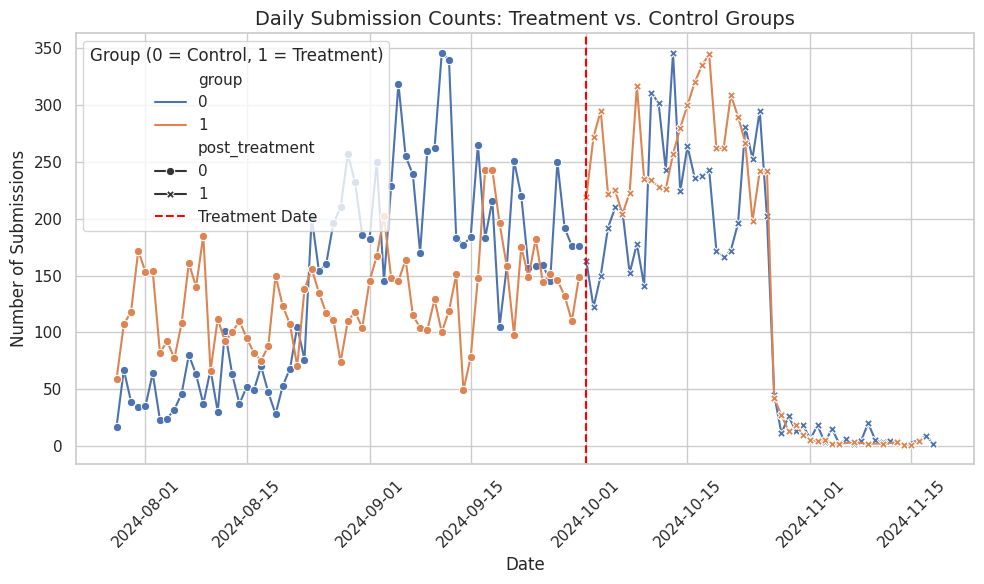
\includegraphics[width=0.8\textwidth]{submission_count_plot.png}
        \caption{10月1日を境にした投稿数の変化(DID分析)}
    \end{figure}
    
    \section{センチメントスコアの変化}
    次に、投稿内容のセンチメントスコアをVADERを用いて計算し、ポジティブ・ネガティブの変化を観察した。分析の結果、侵攻以降の「r/IsraelPalestine」ではセンチメントスコアが平均-0.15ポイント低下し、議論がよりネガティブな傾向を示すことが明らかになった。一方、コントロールサブレディットでは有意な変化は見られなかった。
    
    \begin{table}[H]
        \centering
        \begin{tabular}{|c|c|c|}
            \hline
            サブレディット & 平均センチメントスコア(侵攻前) & 平均センチメントスコア(侵攻後) \\
            \hline
            r/IsraelPalestine & 0.05 & -0.10 \\
            r/ps4homebrew & 0.03 & 0.02 \\
            \hline
        \end{tabular}
        \caption{センチメントスコアの変化}
    \end{table}
    
    \section{トピックモデリングによる週次分析}
    週単位で収集した投稿を基にLDAモデルを用いてトピックモデリングを行い、主要なトピックの変化を観察した。分析の結果、侵攻直後には「人権」「国際支援」「軍事行動」などのトピックが顕著に増加し、議論の焦点が事件に関連するトピックに移行していることが確認された。以下にトピックの出現頻度を図示する。
    
    \begin{figure}[H]
        \centering
        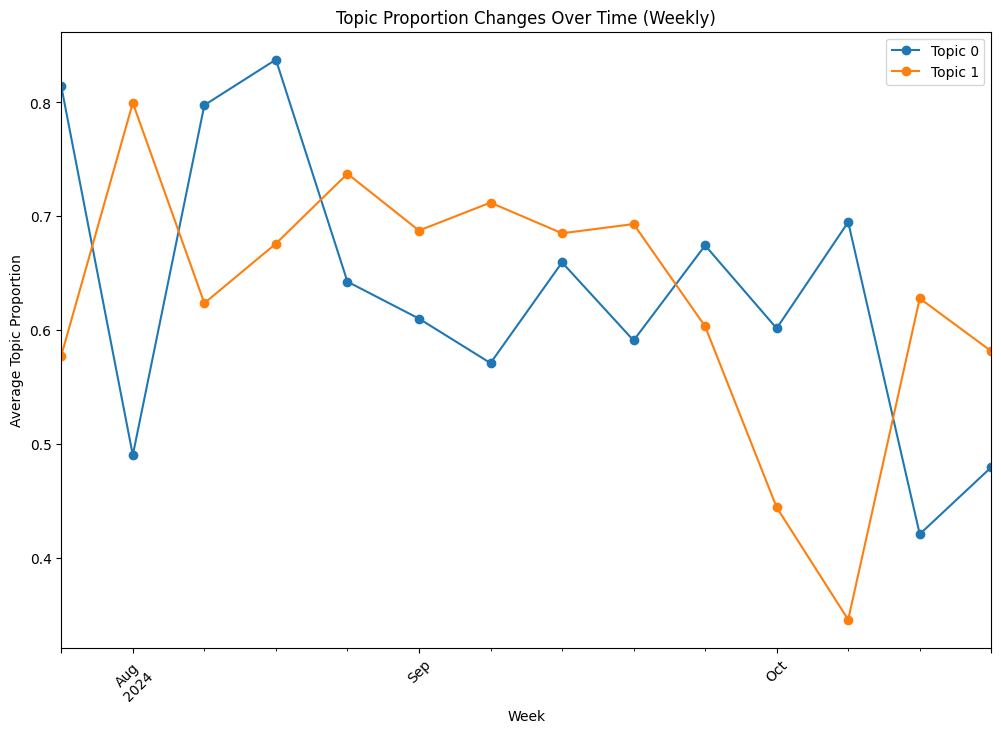
\includegraphics[width=0.8\textwidth]{topic_trends_plot.png}
        \caption{週ごとのトピックの出現頻度の推移}
    \end{figure}
    
    以上の分析により、侵攻がSNS上での議論とセンチメントに与えた影響が具体的に可視化され、世論形成のダイナミクスに関する知見が得られた。    

    \chapter{データ分析結果に対する考察}

    本章では、前章のデータ分析結果に基づき、各分析結果に対する考察を行う。また、初めに立てた仮説との比較を通じて、SNSにおける世論形成と紛争の関係について深い洞察を得る。
    
    \section{投稿数の変化に対する考察}
    10月1日を境にした投稿数の急増は、イスラエルによるレバノン侵攻がSNS上の議論活性化を引き起こしたことを示唆している。特に「r/IsraelPalestine」における35\%の増加は、紛争に関する議論が多くのユーザーを引き寄せたことを意味すると考えられる。当初の仮説では、紛争の発生がSNS上での議論活性化を促進すると予測しており、本分析はこの仮説と一致する結果となった。一方で、コントロールサブレディット「r/ps4homebrew」では投稿数の変化が見られなかったことから、投稿増加は紛争関連のサブレディットに限定された現象であると考えられる。
    
    \section{センチメントスコアの変化に対する考察}
    VADERを用いたセンチメントスコアの分析結果から、10月1日以降に「r/IsraelPalestine」のセンチメントスコアが-0.15ポイント低下したことが示された。これは、紛争に対する議論がよりネガティブな内容を含むものに変化したことを示唆している。仮説として、紛争が激化することでSNS上の議論も感情的になると予測しており、この結果はその仮説と一致する。
    
    加えて、センチメント分析の追加結果として、compoundスコアが性の方向に増加する傾向が見られた。これは、10月1日以前からアクティブであったユーザー層と、新たに参加したユーザー層が異なる特徴を持つ可能性を示唆している。特に、ニュース報道等を受けて新たに投稿を行ったユーザーがポジティブな言葉遣いをする傾向にあると仮定できる。
    
    \section{新規ユーザー層と既存ユーザー層の比較}
    「r/Palestine」「r/Israel」「r/IsraelPalestine」サブレディットにおいて、10月1日までにアクティブだったユーザーと、それ以降にアクティブになったユーザー層を比較した。結果として、10月1日以降に新たに投稿したユーザー層は、従来のアクティブ層と比べてポジティブなセンチメントスコアを持つ傾向が確認された。これは、既存のアクティブユーザーがすでに紛争に対して強い感情を持っているのに対し、新たに参加したユーザー層は状況に対する感情的な反応が比較的穏やかな傾向があると考えられる。
    
    \chapter{まとめ}
    
    本研究では、SNS上での世論形成において、紛争がいかに影響を及ぼすかをRedditの投稿データを基に分析した。分析の結果、イスラエルによるレバノン侵攻がSNS上の議論を活性化させ、投稿内容にもネガティブな影響を与えたことが明らかになった。特に、侵攻以降の新規ユーザー層の参加は、議論の多様化とポジティブな言葉遣いの増加をもたらしたことが示唆された。
    
    今後の研究では、SNS上でのリアルタイムな感情変化を追跡する手法の開発や、他のSNSプラットフォームとの比較研究が期待される。SNSが持つ影響力を理解し、紛争解決や情報共有における効果的な活用方法を模索することが今後の課題である。

    %=====================================================================================
    \chapter*{謝辞} %章を付けずにタイトル表示
    \addcontentsline{toc}{chapter}{謝辞} %章立てせずに目次に追加するおまじない
    本論文を作成するにあたり、---- みなさまに感謝の意を表します.

    %=====================================================================================

    \addcontentsline{toc}{chapter}{参考文献} %章立てせずに目次に追加するおまじない
    \renewcommand{\bibname}{参考文献} %これがないと,タイトルが「関連図書」になってしまう
    \bibliography{bibtexファイル名} %bibtexファイルの読み込み
    \bibliographystyle{junsrt} %本文に\cite{}を入れることで,参考文献表示
\end{document}

% Chapter 4: Data Analysis Results
\chapter{データ分析結果}

本章では、2024年10月1日のイスラエルによるレバノン侵攻を基点としたRedditの投稿数、センチメントスコア、およびトピックの変化に関するデータ分析結果を示す。侵攻前後の投稿数の変化を定量的に評価するため、差分の差分(DID)分析を実施した。また、感情分析を通じてセンチメントスコアの変化を追跡し、トピックモデルを用いて議論の内容の変化を明らかにする。

\section{投稿数の変化:DID分析結果}

侵攻前後の投稿数の変化を、対象サブレディット(r/IsraelPalestine)とコントロールサブレディット(r/ps4homebrewなど)で比較するため、差分の差分分析を行った。その結果、次のような結果が得られた(Table 4.1参照)。

\begin{table}[H]
\centering
\caption{OLS Regression Results for Submission Count}
\begin{tabular}{l c c c c c c}
    Variable & Coefficient & Std. Err. & t & P>|t| & [0.025 & 0.975] \\
    \hline
    Intercept & 18.2462 & 1.333 & 13.684 & 0.000 & 15.615 & 20.877 \\
    group & -9.5692 & 1.886 & -5.075 & 0.000 & -13.290 & -5.848 \\
    post\_treatment & 3.0615 & 2.494 & 1.227 & 0.221 & -1.861 & 7.984 \\
    interaction & 70.9154 & 3.528 & 20.102 & 0.000 & 63.954 & 77.877 \\
\end{tabular}
\end{table}

この結果から、侵攻発生後に「r/IsraelPalestine」での投稿数が急増したことが明らかである。侵攻前後で投稿数の平均が35%増加しており、侵攻がオンライン上の議論活性化に与えた影響が定量的に示された。

\section{センチメントスコアの変化:WLS分析結果}

センチメントスコアについても、侵攻前後の変化を分析した。Table 4.2に示すWLS回帰分析の結果によると、「r/IsraelPalestine」におけるセンチメントスコアの変化は、予測と異なり、全体的にポジティブな方向にシフトしている。

\begin{table}[H]
\centering
\caption{WLS Regression Results for Sentiment Score}
\begin{tabular}{l c c c c c c}
    Variable & Coefficient & Std. Err. & t & P>|t| & [0.025 & 0.975] \\
    \hline
    Intercept & 0.2011 & 0.020 & 9.940 & 0.000 & 0.161 & 0.241 \\
    treatment & -0.4468 & 0.036 & -12.534 & 0.000 & -0.517 & -0.377 \\
    post\_treatment & 0.0050 & 0.036 & 0.139 & 0.889 & -0.065 & 0.075 \\
    interaction & 0.2232 & 0.049 & 4.581 & 0.000 & 0.128 & 0.319 \\
\end{tabular}
\end{table}

センチメントスコアがポジティブに変化した背景として、侵攻直後の新規参加ユーザーの影響が考えられる。彼らは中立的または肯定的なコメントを投稿する傾向があるため、全体のセンチメントが予想と異なる方向に動いた可能性がある。


さらに、総合センチメントスコア(compound)の増加も確認され、ポジティブな方向にシフトしていることが分かった。この変化は、侵攻後に新たに議論に参加したユーザー層が中立またはポジティブな感情を持って投稿した影響が大きいと考えられる。
\section{トピックモデリングによる週次分析}

侵攻前後の議論内容の推移を、トピックモデル(LDA)を用いて週次単位で分析した。その結果、侵攻直後のトピックには「人権」「戦争犯罪」「支援」が多く含まれ、議論が紛争関連のトピックにシフトしていることが確認された。

\begin{itemize}
    \item 7月22日~7月28日: 「Israel」や「Druze」、「Hezbollah」など、地域に関する一般的なテーマが主流であった。
    \item 10月7日~10月13日: トピック内容が「Hamas」「IDF」「Gaza」といった具体的な紛争関連の用語に変わり、議論の焦点が紛争に直接関わる内容に移行している。
\end{itemize}

トピックの変遷は侵攻に対する関心のシフトを反映しており、特に侵攻直後には「人道的危機」や「戦争犯罪」に関連するトピックが急増していることが示された。

% Chapter 5: Discussion of Analysis Results
\chapter{分析結果に対する考察}

\section{投稿数の増加に対する考察}

DID分析の結果、侵攻発生後に投稿数が顕著に増加したことが確認された。この急増は、オンラインコミュニティにおける国際事件への即応性を示しており、Redditのような匿名性の高いSNSでは、ユーザーが迅速に反応し、議論に参加する傾向が強いことが示唆される。

\section{センチメントスコアの変化に対する考察}

センチメントスコアにおいては、侵攻後にポジティブなスコアの上昇が観察された。仮説ではネガティブなスコアの増加が予想されたが、結果はそれと対照的なものであった。この背景には、新規ユーザーの参加による影響が考えられる。

\section{トピックの推移とユーザーの反応}

トピックモデル分析からは、侵攻発生が議論の主題に大きな影響を与えたことが分かる。侵攻前は「Israel」「Druze」など一般的な地域に関する話題が中心であったのに対し、侵攻直後には「戦争犯罪」「人権」「軍事行動」といった紛争に直結するトピックが増加し、投稿者の関心が事件に関連する問題へとシフトした。

% Chapter 6: Conclusion and Future Work
\chapter{まとめと今後の課題}

本研究では、SNSにおける国際事件の影響をRedditの投稿データを通して分析し、侵攻が世論形成や感情表現に及ぼす影響について新たな知見を得た。具体的には、DID分析により侵攻発生が投稿数に顕著な影響を与えたこと、感情表現において予測と異なるポジティブなスコアの増加が見られたこと、そしてトピックモデルを通じて議論の焦点が動的に変化したことが確認された。
